\documentclass{subfiles}

\usepackage{graphicx}
\usepackage{amsfonts}
\usepackage{amssymb}
\usepackage{amsmath}

\graphicspath{ {fisica-generale/assets/} }

\begin{document}

\section{Cinematica}

La cinematica è lo studio moto. Il moto dipende dal sistema di riferimento.

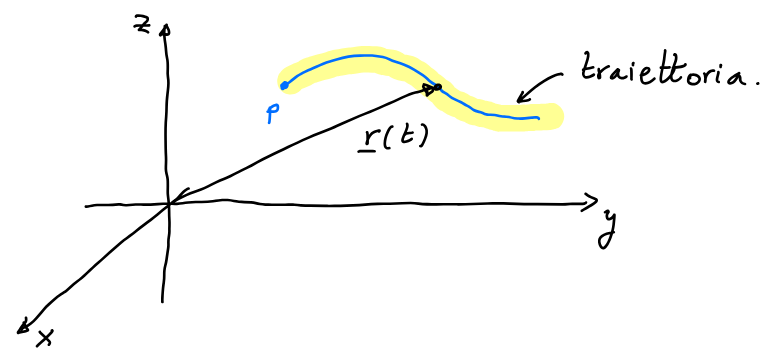
\includegraphics[width=\columnwidth]{moto-di-un-punto}

\noindent
Possiamo descrivere il moto di un punto materiale come una funzione.

$$
\begin{matrix}
r: &\mathbb{R} &\to &\mathbb{R}^3 \\
&t &\to &\vec{r}(t)
\end{matrix}
$$

\subsection{Punto}

\subsubsection{Definizione}

Dato $\vec{r}(t)$ che descrive il moto di un punto, definiamo la traiettoria come il luogo dei punti dello spazio "esplorati" da $\vec{r}(t)$ al variare di $t$.

\noindent
$\vec{r}(t)$ è un vettore dimensionale:

$$
\vec{r}(t) = (r_x(t), r_y(t), r_z(t))
$$

\subsubsection{Notazione}

$$
[r_x] = (m)
$$

\subsection{Velocità}

\subsubsection{Definizione}

La velocità è una funzione vettoriale che associa ad ogni tempo "lo spostamento infinitesimo" in un intervallo di tempo infinitesimo.

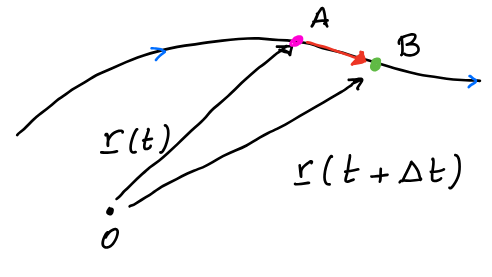
\includegraphics[width=\columnwidth]{rappresentazione-velocita-grafica}

$$
\vec{v}(t) = \lim_{\Delta t \to 0} \frac{\vec{r}(t + \Delta t) - \vec{r}(t)}{\Delta t} = \frac{d}{dt} \vec{r}(t)
$$

\noindent
$\vec{v}(t)$ è un vettore che possiamo esprimere in componenti

$$
\vec{v}(t) = (v_x(t), v_y(t), v_z(t))
$$

\noindent
Perciò:

$$
\begin{matrix}
\vec{r}(t) = (r_x(t), r_y(t), r_z(t)) \\
v_x(t) = \frac{d}{dt} r_x(t) \\
v_y(t) = \frac{d}{dt} r_y(t) \\
v_z(t) = \frac{d}{dt} r_z(t)
\end{matrix}
$$

\subsubsection{Notazione}

La velocità si misura in $m/s$

\subsubsection{Proprietà della derivata}

1) $\frac{d}{dt}(\vec{f}(t) + \vec{g}(t)) = \frac{d}{dt}\vec{f}(t) + \frac{d}{dt}\vec{g}(t)$
2) Sia $\lambda(t)$ una funzione reale in $\mathbb{R}$ e $\vec{f}(t) \in \mathbb{R}^3$: $\frac{d}{dt}(\lambda(t)\vec{f}(t)) = (\frac{d}{dt}\lambda(t))\vec{f}(t) + \lambda(t)(\frac{d}{dt}\vec{f}(t))$
3) Siano $\vec{f}(t), \vec{g}(t) \in \mathbb{R}^3$, allora: $\frac{d}{dt}(\vec{f}(t)\vec{g}(t)) = (\frac{d}{dt}\vec{f}(t))\vec{g}(t) + \vec{f}(t)(\frac{d}{dt}\vec{g}(t))$
4) $\frac{d}{dt}(\vec{f}(t) \wedge \vec{g}(t)) = (\frac{d}{dt}\vec{f}(t)) \wedge \vec{g}(t) + \vec{f}(t) \wedge (\frac{d}{dt}\vec{g}(t))$

\subsection{Accelerazione}

\subsubsection{Definizione}

Dato $\vec{r}(t)$ con velocità $\vec{v}(t)$, definiamo l'accelerazione come:

$$
\vec{a}(t) = \lim_{\Delta t \to 0} \frac{\vec{v}(t + \Delta t) - \vec{v}(t)}{\Delta t} = \frac{d}{dt} \vec{v}(t) = \frac{d^2}{dt^2} \vec{r}(t)
$$

\noindent
Graficamente, la velocità è sempre tangente alla traiettoria.

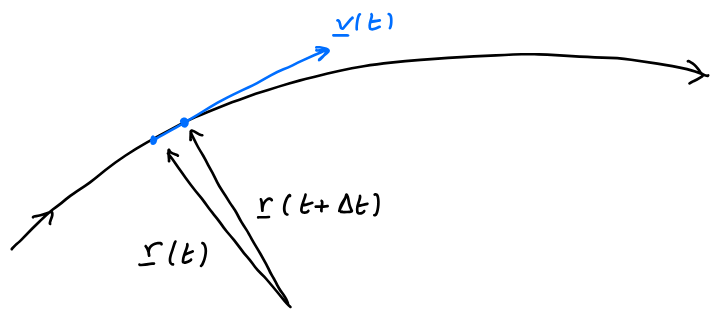
\includegraphics[width=\columnwidth]{rappresentazione-accelerazione-grafica}

\noindent
Si può identificare graficamente l'accelerazione come differenza dei vettori $\vec{v}(t)$ e $\vec{v}(t + \Delta t)$ per $\Delta t$ "piccolo"

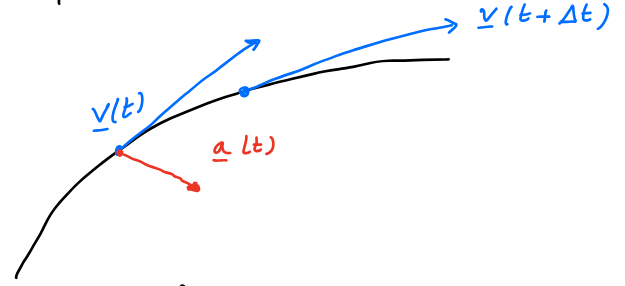
\includegraphics[width=\columnwidth]{rappresentazione-accelerazione-grafica-differenza}

\noindent
Perciò vale la formula (si usa $\simeq$ poiché $\Delta t$ è finito):

$$
\vec{a}(t) \simeq \frac{\vec{v}(t + \Delta t) - \vec{v}(t)}{\Delta t}
$$

\noindent
che graficamente è:

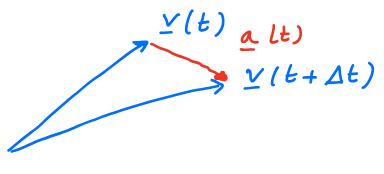
\includegraphics[width=\columnwidth]{rappresentazione-accelerazione-grafica-approssimazione}

\subsection{Il "problema inverso"}

Capita molto più spesso di avere informazioni su $\vec{v}(t)$ o $\vec{a}(t)$ e di voler ricostruire $\vec{r}(t)$. Questo è definito come il "problema inverso" della cinematica, che si riconduce alla risoluzione di equazioni differenziali

\subsubsection{Rappresentazione intrinseca del moto}

Si possono introdurre una serie di elementi per caratterizzare il moto in modo "intrinseco", cioè indipendente dal sistema di riferimento. Il primo concetto presentato è quello della ascissa curvilinea

\subsubsection{Ascissa curvilinea}

L'ascissa curvilinea, $s(t)$, è la lunghezza della traiettoria percorsa fino al tempo $t$.

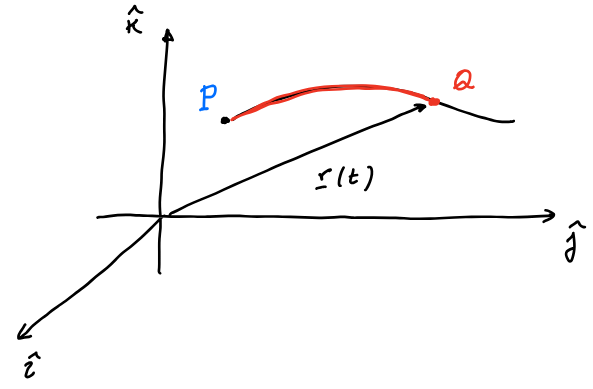
\includegraphics[width=\columnwidth]{ascissa-curvilinea}

$$
\begin{matrix}
s(t) &\simeq& \sum_{t'} |\vec{r}(t' + \Delta t) - \vec{r}(t')| \\
&\simeq& \sum_{t'} \Delta t |\vec{v}(t')| \\
&=& \int^{t}_{0}{dt' |\vec{v}(t)|}
\end{matrix}
$$

\end{document}
